\setcounter{section}{21}
\setcounter{theorem}{21}
\section*{21 + 22 Riesz-Markow Theorem \tiny(21, p. [243-249], \cite{schilling2017measures})}
Assume \((X,d)\) is a locally compact metric space. 
\begin{definition}[\colordefinition{positive linear functional}]
    A linear functional \(\rho:C_c(X)\rightarrow\mathbb{C}\) is called positive if \(\rho(f)\geq0\) for all \(f\geq0\). (Recall \(C_c(X)\) is the space of continuous (C) compactly supported (c) functions.)
\end{definition}
\begin{theorem}[\ifcolor\color{red}\textbf{Riesz-Markov}\color{black}\else Riesz-Markov\fi]
    If \(\rho:C_c(X)\rightarrow \mathbb{C}\) is a positive linear functional, where \((X,d)\) is a locally compact metric space, then there exists a Borel measure \(\mu\) on \(X\) s.t. \(\mu(K)<\infty\) for every compact \(K\subset X\) and
    \begin{align*}
        \rho(f) = \int_X f d\mu \ \forall f\in C_c(X).
    \end{align*}
    If \(X\) is separable, then such a measure \(\mu\) is unique. 
\end{theorem}
For the proof we need two auxiliary results.
\begin{lemma}[Urysohn's Lemma]
    Assume \((X,d)\) is a metric space, \(A,B\subset X\) are disjoint closed subsets. Then there exists a continuous function \(f:X\rightarrow[0,1]\) s.t. \(f\equiv1\) on \(A\) and \(f\equiv0\) on \(B\).
\end{lemma}
\ifdetailed
\begin{proof}
    Define,
    \begin{align*}
        f(x) = \frac{d(x,B)}{d(x,A)+d(x,B)}.
    \end{align*}
    Note that this is well-defined, since
    \(d(x,A) + d(x,B)>0\) for all \(x\), as \(\{x:d(x,A)=d(x,B)=0\} = A\cap B = \emptyset\).
\end{proof}
\fi
\begin{lemma}
    Assume \((X,d)\) is a compact metric space, \(U=(U_i)_{i=1}^{n}\) is a finite open cover of \(X\) (so \(U_i\) are open and \(\cup_{i=1}^{n}U_i = X\)). Then there exist functions \(\rho_1, ..., \rho_n\) in \(C(x)\) s.t.
    \begin{align*}
        0\leq \rho_i\leq 1, \ \text{supp}(\rho_i)\subset U_i, \ \sum\limits_{i=1}^{n}\rho_i(x)=1 \ \forall x.
    \end{align*}
    Every such collection of functions is called a \colordefinition{partition of unity subordinate } to \(U\).
\end{lemma}
\ifdetailed
\begin{proof}
    Let us show first that there exists an open set \(V_1\) s.t. \(\bar{V}_1\subset U_1\) and \(X=V_1\cup U_2\cup ... \cup U_n\). For this, consider the closed set \(K=X\backslash\left(U_2\cup ... \cup U_n\right) \subset U_1\). For every \(x\in K\) we can find a ball \(B_{r_x}(X)\) (\(r_x>0\)) s.t. \(B_{r_x}(x)\subset U_1\). As \(K\) is compact and \((B_{r_x}(x))_{x\in K} \) is an open covert of \(K\), we can find a finite subcover \((B_{r_x}(x_k))_{k=1}^{m}\). Then put \(V_1 = \cup_{k=1}^{m}B_{r_{x_k}}(x_k)\). Using this construction \(2n\) times we can find open sets \(V'_1, ..., V'_n\) and \(V''_1, ..., V''_n\) s.t. \(\bar{V}'_i\subset V''_{i}, \bar{V}''_{i}\subset U_i\), \(\cup_{i=1}^{n}V'_i = X\). By Urysohn's lemma, for every \(i\), we can find \(f_i\in C(X)\) s.t. \(0\leq f_i\leq 1\), \(f_i\equiv 1\) on \(\bar{V}'_i\), \(f_i\equiv 0\) on \(X\backslash V''_i\). Then supp\((f_i)\subset \bar{V}''_j\subset U_j\). Define
    \begin{align*}
        \rho_i(x) = \frac{f_i(x)}{\sum_{j=1}^{n}f_j(x)}.
    \end{align*}
\end{proof}
\fi
\ifdetailed
\begin{proof}[Proof of the Riesz-Markov Theorem]
    Assume \(\phi:C_c(X)\rightarrow\mathbb{C}\) is positive for open \(U\subset X\), define
    \begin{align*}
        \mu(U) \eqdef \sup\left\{\phi(f): 0\leq f\leq 1, \text{supp}(f) \subset U\right\}.
    \end{align*}
    For a set \(A\subset X\), define then 
    \begin{align*}
        \mu^*(A) \eqdef \inf_{\substack{A\subset U \\ U\text{ open}}}\mu(U).
    \end{align*}

    \textbf{Step 1}. \(\mu^*\) is an outer measure on \(X\) and \(\mu^*(U)=\mu(U)\) for open \(U\). Observe first that if \(V\subset U\) is open, then \(\mu(V)\leq\mu(U)\). This implies that \(\mu^*(V)=\mu(V)\) for all open \(V\). Obviously, \(\mu^*(\emptyset)=\mu(\emptyset)=0\). We need to show that 
    \begin{align*}
        \mu^*\left(\bigcup\limits_{n=1}^{\infty}A_n\right) \leq \sum\limits_{n=1}^{\infty} \mu^*(A_n).
    \end{align*}
    We may assume that \(\mu^*(A_n)<\infty\) for all \(n\), as otherwise there is nothing to prove.

    Assume first that \(A_n=U_n\) are open. Take \(f\in C_c(X)\) with \(0\leq f\leq 1\) s.t. \(\text{supp}(f)\subset\cup_{n\in\mathbb{N}}U_n\). As supp\((f)\) is compact, there is a \(N\) s.t. supp\((f)\subset \cup_{n=1}^{N}U_n\). Let \(\rho_1, ..., \rho_N\) be a partition of unity  in \(C(\text{supp}(f))\) subordinate to \((U_n\cap\text{supp}(f))_{n=1}^{N}\). Define
    \begin{align*}
        f_n(x) = \begin{cases}
            \rho_n(x)f(x), \text{ if } x\in\text{supp}(f), \\
            0, \text{ otherwise}
        \end{cases}.
    \end{align*}
    Note that the functions \(f_n\) are continuous. 

    \(\Big(\)Indeed, if \(x\notin \text{supp}(f)\) or \(x\in\inf(\text{supp}(f))\), then \(f(y)\rightarrow f(x)\) as \(y\rightarrow x\), as 0 is continuous on \(X\backslash\text{supp}(f)\) and \(\rho_n,f\) are continuous on \(\inf(\text{supp}(f))\). Assume now that \(x\in(\text{supp}(f))\backslash\inf(\text{supp}(f))\), so \(x\in\text{supp}(f)\), but \(B_r(x)\backslash\text{supp}(f)\neq\emptyset \ \forall r>0\). Then \(f(x) = 0\) and \(f(y)\rightarrow 0 \) as \(y\rightarrow x\), since
    \begin{align*}
        \lim_{\substack{y\rightarrow x \\ y\in\text{supp}(f)}} \rho_n(y)f(y) = \rho_n(x)f(x) = 0. \Big)
    \end{align*}
    Note also that 
    \begin{align*}
        \text{supp}(f_n) < \text{supp}(\rho_n) \subset U_n.
    \end{align*}
    Hence, \(\phi(f_n)\leq \mu(U_n)\). Therefore
    \begin{align*}
        \phi(f) = \sum\limits_{n=1}^{N}\phi(f_n) \leq \sum\limits_{n=1}^{N}\mu(U_n) \leq\sum\limits_{n=1}^{\infty} \mu(U_n).
    \end{align*}
    Taking the supremum over all \(f\)  s.t. \(0\leq f\leq 1\), supp(f) \(\subset \cup_{n\in\mathbb{N}}U_n\), we set
    \begin{align*}
        \mu\left(\bigcup\limits_{n=1}^{\infty}U_n\right) \leq \sum\limits_{n=1}^{\infty}\mu(U_n).
    \end{align*}
    
    For general \(A_n\), fix \(\epsilon>0\) and choose open \(U_n\) s.t. 
    \begin{align*}
        A_n\subset U_n \text{ and } \mu(U_n)<\mu^*(A_n) + \frac{\epsilon}{2^n}.
    \end{align*}
    Then
    \begin{align*}
        \mu^*\left(\bigcup\limits_{n=1}^{\infty}A_n\right) \leq \sum\limits_{n=1}^{\infty}\mu^*(A_n).
    \end{align*}
    This completes step 1.

    \textbf{Step 2}. All Borel sets are Caratheodory measurable (with respect to \(\mu^*\)). It suffices to show that every open set \(U\) is Caratheodory measurable. We need to check that 
    \begin{align*}
        \mu^*(A) \geq \mu^*\left(A\cap U\right) + \mu^*\left(A\cap U^c\right) \ \forall A\subset X.
    \end{align*}
    Consider first an open set \(A=V\). We may assume that \(\mu(V)<\infty\), as otherwise there is nothing to prove. 

    Fix \(\epsilon>0\) and choose \(f\) s.t.
    \begin{align*}
        0\leq f\leq 1, \text{supp}(f)\subset V\cap U, \phi(f)>\mu\left(V\cap U\right) - \epsilon.
    \end{align*}
    Consider the open set \(W=V\backslash\text{supp}(f)\).

    Choose \(0\leq g\leq 1\), supp\((g)\subset W\), \(\phi(g)>\mu(W)-\epsilon\). Then
    \begin{align*}
        \mu\left(V\cap U\right) + \mu^*\left(V\cap U^c\right) &\leq \mu\left(V\cap U\right) + \mu(W) \\
        &< \phi(f) + \phi(g) + 2\epsilon = \phi(f+g) + 2\epsilon \\
        &\leq \mu(V) + 2\epsilon,
    \end{align*}
    since \(0\leq f+g\leq 1\), supp\((f+g)\subset V\). As \(\epsilon>0\) was arbitrary, we get the required inequality. 

    For general \(A\), take \(V\supset A\), \(V\) open. Then 
    \begin{align*}
        \mu(V) \geq \mu\left(V\cap U\right) + \mu^*\left(V\cap U^c\right) \geq \mu^*\left(A\cap U\right) + \mu^*\left(A\cap U^c\right).
    \end{align*}
    Taking the infimum over all \(V\) we get
    \begin{align*}
        \mu^*(A) \geq \mu^*\left(A\cap U\right) + \mu^*\left(A\cap U^c\right).
    \end{align*}
    
    \subsection*{Lecture 22}
    \setcounter{section}{22}
    \setcounter{theorem}{22}

    \textbf{Step 3}. If \(K\subset X\) is compact, then \(\mu(K)<\infty\) and \\ \(\mu(K)=\inf\{\phi(f):\vmathbb{1}_K\leq f\}\). Also, if \(0\leq f\leq \vmathbb{1}_K\), then \(\phi(f)\leq\mu(K)\).

    Assume \(\vmathbb{1}_K\leq f\). Fix \(\epsilon>0\) and consider the open set \(U=\{x:f(x)>1-\epsilon\}\). Assume \(0\leq g\leq 1\), supp\((g)\subset U\). Then \(g\leq f/(1-\epsilon)\), hence \(\phi(g)\leq \phi(f)/(1-\epsilon)\). Taking the supremum over all such \(g\), we get \(\mu(U)\leq \phi(f)/(1-\epsilon)\). Hence
    \begin{align*}
        \mu(K) \leq\mu(U)\leq\phi(f)/(1-\epsilon).
    \end{align*}
    As \(\epsilon>0\) was arbitrary, we get \(\mu(K)\leq\phi(f)\). In particular, \(\mu(K)<\infty\). (Note that \(f\in C_c(X)\) s.t. \(\vmathbb{1}_K\leq f\) exists by Usysohn's lemma.) We see also that 
    \begin{align*}
        \mu(K)\leq \int\left\{\phi(f):\vmathbb{1}_K\leq f\right\}.
    \end{align*}

    In order to prove the equality, fix \(\epsilon>0\) and choose an open \(U\) s.t.
    \begin{align*}
        K\subset U, \ \mu(K)>\mu(U)-\epsilon.
    \end{align*}
    By Urysohn's lemma we can find \(f\in C_c(X)\) s.t. \(0\leq f\leq 1\), \(f\equiv 1\) on \(K\) (so \(\vmathbb{1}_K\leq f\)) and supp\((f)\subset U\). Then
    \begin{align*}
        \phi(f)\leq\mu(U)<\mu(K) + \epsilon.
    \end{align*}
    Therefore,
    \begin{align*}
        \inf\left\{\phi(f):\vmathbb{1}_K\leq f\right\}.
    \end{align*}
    Finally, assume \(0\leq f\leq\vmathbb{1}_K\). Then for every open \(U\supset K\) we have supp\((f)\subset U\), so \(\phi(f)\leq\mu(U)\). Hence
    \begin{align*}
        \phi(f) \leq \inf_{\substack{K\subset U \\ U \text{ open}}} \mu(U) = \mu(K).
    \end{align*}

    \textbf{Step 4}. \(\phi(f) = \int_X fd\mu\ \forall f\in C_c(X)\). 

    It suffices to consider \(0\leq f\leq 1\), as such functions span \(C_c(F)\). Consider \(K=\text{supp}(f)\) and define for some \(N\),
    \begin{align} 
        K_n &= \left\{ x\in K:f(x) \geq \frac{n}{N} \right\} \ (n=0, ..., N), \\ \label{eq:f_n1289070}
        f_n(x) &= \min\left\{f(x), \frac{n}{N} \ \right\}, \ (n=0, ..., N), \\
        g_n(f) &= f_n(x)-f_{n-1}(x),  \ (n=1, ..., N).
    \end{align}
    Then \(f_0 = 0, \ f_N=f\), so \(f=\sum_{n=1}^{N}g_n\).
    \begin{figure}[H]
        \centering 
        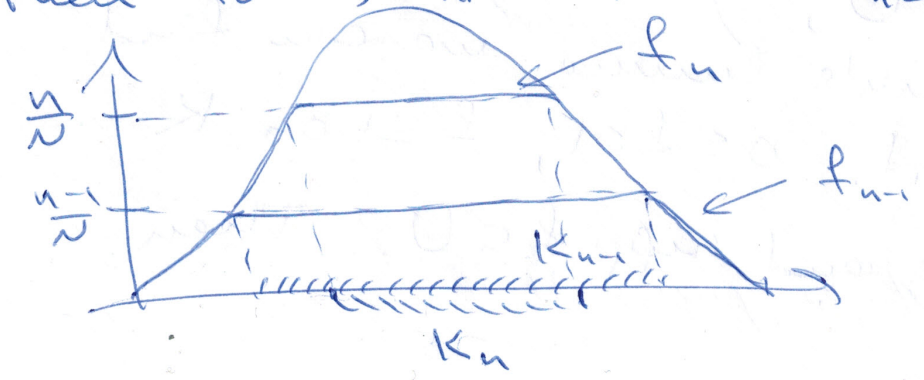
\includegraphics[scale=0.5]{Figs/f_ns_proof_RM.png}
        \caption{Drawing of the \(f_n\)'s defined in eq. (\ref{eq:f_n1289070}).}
    \end{figure}
    We have
    \begin{align*}
        \frac{1}{N}\vmathbb{1}_{K_n} \leq g_n \leq \frac{1}{N}\vmathbb{1}_{K_{n-1}} \ (n=1, ..., N).
    \end{align*}
    By integrating we get
    \begin{align*}
        \frac{1}{N}\mu(K_n) \leq \int_X g_n d\mu\leq \frac{1}{N} \mu(K_{n-1}).
    \end{align*}
    On the other hand, by step 3 we have
    \begin{align*}
        \frac{1}{N}\mu(K_n) \leq \phi(g_n) \leq \frac{1}{N} \mu(K_{n-1}).
    \end{align*}
    It follows that both \(\int_X fd\mu\) and \(\phi(f)\) lie in the interval
    \begin{align*}
        \left[\frac{1}{N}\sum\limits_{n=1}^{N}\mu(K_n), \frac{1}{N}\sum\limits_{n=1}^{N}\mu(K_{n-1})\right].
    \end{align*}
    The length of this interval is
    \begin{align*}
        \frac{1}{N}\left(\mu(K_0) - \mu(K_n)\right) \leq \frac{1}{N} \mu(K_0) = \frac{\mu(K)}{N}.
    \end{align*}
    Therefore,
    \begin{align*}
        \Big\vert \int_X fd\mu - \phi(f) \Big\vert \leq \frac{\mu(K)}{N}.
    \end{align*}
    Letting \(N\rightarrow\infty\) we conclude that
    \begin{align*}
        \phi(f) = \int_X fd\mu.
    \end{align*}

    \textbf{Step 5}. If \(X\) is separable, then \(\mu\) is uniquely determined by \(\phi\).

    Assume \(\mu\) is a Borel measure s.t. \(\mu(K)<\infty\ \forall\) compact \(K\subset X\) and 
    \begin{align*}
        \phi(f) = \int_X f d\mu \ \forall f\in C_c(X).
    \end{align*}
    Recall from the lecture on regularity of measures that then \(\mu\) is regular (as \(X\) is separable, locally compact). In particular,
    \begin{align*}
        \mu(A) = \inf_{\substack{A\subset U \\ U \text{ open}}} \mu(U) \ \forall A\in \mathscr{B}(X).
    \end{align*}
    Therefore it suffices to show that \(\mu(U)\) is determined by \(\phi\).

    If \(\bar{U}\) is compact, then \(f_n\nearrow \vmathbb{1}_U\), where
    \begin{align*}
        f_n(x) = \frac{n d(x,U^c)}{1 + nd(x,U^c)}.
    \end{align*}
    Hence,
    \begin{align*}
        \mu(U) = \lim\limits_{n\rightarrow\infty}\int_X f_n d\mu = \lim\limits_{n\rightarrow\infty} \phi(f_n).
    \end{align*}
    For general \(U\), we can find open \(U_n\) s.t. \(\bar{U}_n\) are compact and \(U_n\uparrow U\) (again, recall the lecture on regularity). Then \(\mu(U_n)\nearrow\mu(U)\), so \(\mu(U)\) is determined by \(\phi\).
\end{proof}
\fi
\begin{remark}
    Without separability, the uniqueness is not always true. It can be checked that the measure we constructed in the proof,
    \begin{align*}
        \mu(U) \eqdef \sup\left\{\phi(f): 0\leq f\leq 1, \text{supp}(f) \subset U\right\},
    \end{align*}
    has the following properties:
    \begin{enumerate}[label=(\roman*)]
        \item \(\mu(K)<\infty\) \(\forall\) compact \(K\subset X\);
        \item \(\mu\) is outer regular \((\mu(A)=\inf_{\substack{A\subset U\\ U\text{ open}}} \mu(U))\);
        \item \(\mu\) is inner regular on open sets (this is where we need the full strength of step 3):
        \begin{align*}
            \mu(U) = \sup_{\substack{K\subset U \\ K \text{ compact}}} \ \forall \text{ open }U.
        \end{align*}
    \end{enumerate}
    Such measures are called \colordefinition{Radon measures}. It can be shown that the uniqueness holds within the class of Radon measures.
\end{remark}
\subsection*{Dual of \(\boldsymbol{C(X)}\)}
As an application of the Riesz-Markow Theorem we will describe \(C(X)^*\) in terms of measures for compact metric spaces \((X,d)\).

Denote by \(M(X)\) the space of complex Borel measures on \(X\). For every \(\nu\in M(X)\) we want to make sense of \(\int_Xfd\nu\) for \(f\in C(X)\). It is enough to consider finite signed measures, as then we can define
\begin{align*}
    \int_Xfd\nu = \int_Xfd(\text{Re}\nu) + i\int_X fd(\text{Im}\nu).
\end{align*}
So assume \(\nu\) is a finite signed measure. Then, \(\nu=\mu_1 - \mu_2\) for positive measures and we define
\begin{align*}
    \int_Xfd\nu = \int_X fd\mu_1 - \int_Xfd\mu_2.
\end{align*}
This is well-defined, since if
\begin{align*}
    \nu=\mu_1-\mu_2 = \omega_1-\omega_2,
\end{align*}
then \(\mu_1 + \omega_2 = \mu_2 + \omega_1\) and
\begin{align*}
    \int_Xfd\mu_1 + \int_Xfd\omega_2 = \int_Xfd\mu_2 + \int_Xfd\omega_1.
\end{align*}
Thus, every \(\nu\in M(X)\) defines a linear functional
\begin{align*}
    \phi_{\nu} : C(X) \mathbb{C} \text{ by }\phi_{\nu}(f) = \int_xfd\nu,
\end{align*}
and the map \(\nu\mapsto\phi_{\nu}\) is linear.

\begin{lemma}
    If \(\nu\in M(X)\) and \(d\nu = gd|\nu|\) is its polar decomposition, then
    \begin{align*}
        \int_Xfd\nu = \int_X fgd|\nu| \ \forall f\in C(X).
    \end{align*}
\end{lemma}
\ifdetailed
\begin{proof}
    More generally, let us show that if \(\mu\) is a finite Borel measure, \(g\in L^1(X,d\mu)\), and \(d\nu = gd\mu\), then
    \begin{align*}
        \int_X fd\nu = \int_X fgd\mu \ \forall f\in C(X).
    \end{align*}
    
    It suffices to consider \(g\geq 0\). Then \(\nu\) is positive, so \(\int_X fd\nu\) has the usual meaning.

    We will then prove an even more general statement:
    \begin{align*}
        \int_X fd\nu = \int_X fg d\mu \ \forall f\in L^{\infty}(X,\mu).
    \end{align*}
    As simple functions are dense in \(L^{\infty}(X,\mu)\), it suffices to consider simple \(f\), hence it suffices to consider \(f=\vmathbb{1}_A\). Then
    \begin{align*}
        \int_X\vmathbb{1}_Ad\nu = \nu(A)\int_A fd\mu = \int_X \vmathbb{1}gd\mu,
    \end{align*}
    where the second equality comes from the definition of \(d\nu = gd\mu\).
\end{proof}
\fi 
\begin{lemma}
    For every \(\nu\in M(X)\), the linear functional \(\phi_{\nu}\) is bounded and \(||\phi_{\nu}|| = |\nu|(X)\). (Recall that the norm on \(C(X)\) is \(||f|| = \sup_{x\in X}|f(x)|\).)
\end{lemma}
\ifdetailed
\begin{proof}
    We have, with \(d\nu = gd|\nu|\) being the polar decomposition,
    \begin{align*}
        |\phi_{\nu}(f)| &= \Big\vert \int_X fd\nu\Big\vert = \Big\vert\int_X fgd|\nu|\Big\vert \\ 
        &\leq \int_X |f|d|\nu| \leq ||f||\int_Xd|\nu| \\
        &\leq ||f|| |\nu|(X).
    \end{align*}
    Therefore,
    \begin{align*}
        ||\phi_{\nu}|| \leq |\nu|(X).
    \end{align*}

    For the opposite inequality, recall that \(|\nu|\) is regular and \(X(X)\) is dense in \(L^1(X,d|\nu|)\). Hence, we can find \(f_n\in C(X)\) s.t. \(f_n\rightarrow g\) in \(L^1(X,d|\nu|)\). Define
    \begin{align*}
        g_n(x) = \begin{cases}
            f_n(X), \text{ if } |f_n(x)|\leq 1, \\
            \frac{f_n(x)}{|f_n(x)|}, \text{ if } |f_n(x)|>1.
        \end{cases}
    \end{align*}
    Then \(||g_n||\leq 1\) and \(|g-g_n|\leq |f - f_n|\). Therefore, \(||g-g_n||\leq ||g-f_n||_1\xrightarrow[n\rightarrow\infty]{ }0\). We have
    \begin{align*}
        \phi_{\nu}(\bar{f}_n) = \int_X\bar{g}_n gd|\nu|\rightarrow \int_X d|\nu| = |\nu|(X),
    \end{align*}
    since
    \begin{align*}
        \Big\vert \int_X \left(\bar{g}_n g -1\right) d|\nu|\Big\vert &\leq \int_X |\bar{g}_n g-1| d|\nu|\\
        &=\int_X|\bar{g}_n - \bar{g}|d|\nu| = ||g_n - g||_1 \xrightarrow[n\rightarrow\infty]{ } 0,
    \end{align*}
    where the first equality is because \(|g(x)|=1\). Therefore, \(||\phi_{\nu}||\geq \sup\limits_{n}|\phi_{\nu}(\bar{g}_n)|\geq |\nu|(X)\).
\end{proof}
\fi 